\documentclass[letterpaper,12pt]{scrartcl}
\usepackage{epsfig,latexsym,amsmath,amssymb,epic,eepic,psfrag,subfigure,float,euscript,array}
\usepackage[latin1]{inputenc}
\usepackage[margin=24mm]{geometry}
\usepackage{tikz,pgf,pgfplots}
\usepgfplotslibrary{fillbetween}
\usepgfplotslibrary{groupplots}
\usetikzlibrary{decorations, arrows, fit, circuits.plc.ladder}

\usepackage[amssymb]{SIunits}

\newenvironment{exercise}[1][Exercise]{\begin{trivlist} \item[\hskip
    \labelsep {\stepcounter{exerctr}\bfseries #1
      \arabic{exerctr}}]}{\end{trivlist}\vspace{10mm}}

\newcounter{exerctr}
\newcounter{abcctr}[exerctr]

\newcommand{\abc}{\noindent\vspace{1mm}\\ \textbf{
    \stepcounter{abcctr}(\alph{abcctr})\ }}
\newcommand{\bbm}{\begin{bmatrix}}
\newcommand{\ebm}{\end{bmatrix}}
\newcommand{\point}[1]{\hfill \textbf{ (#1p)}\\ \vspace{-5mm}}
\newcommand{\ctrb}{\EuScript{S}}
\newcommand{\Lap}{\mathcal{L}}
\newcommand{\obsv}{\EuScript{O}}
\newcommand{\realdel}{\text{Re}}
\newcommand{\imagdel}{\text{Im}}
\newcommand{\bC}{\mathbb{C}}
\newcommand{\bR}{\mathbb{R}}
\newcommand{\bmpv}{\begin{minipage}[t]}
\newcommand{\bmps}{\begin{minipage}[t]{45mm}}
\newcommand{\bmpm}{\begin{minipage}[t]{90mm}}
\newcommand{\bmpl}{\begin{minipage}[t]{\textwidth}}
\newcommand{\emp}{\end{minipage}}
\newcommand{\mexp}[1]{\ensuremath{\mathrm{e}^{#1}}}

\newcommand{\AxisRotator}[1][rotate=0]{%
    \tikz [x=0.2cm,y=0.60cm,line width=.1ex,-stealth,#1] \draw (0,0) arc (-150:150:1 and 1);%
}

%\addtolength{\topmargin}{-1cm}
%\textheight 22.5cm
%\oddsidemargin 1.3cm
%\evensidemargin 1.3cm

\makeatletter
\newcommand*{\rom}[1]{\expandafter\@slowromancap\romannumeral #1@}
\makeatother

\newcommand*\circled[1]{\tikz[baseline=(char.base)]{
            \node[shape=circle,draw,inner sep=2pt] (char) {#1};}}


\title{Modeling and automation - Test exam}
\author{Kjartan Halvorsen}
\date{}

\begin{document}

\maketitle


\begin{description}
\item[Time] When convenient, but before the exam on Thursday June 9
\item[Place] 
\item[Permitted aids] The single page with your own notes, table of Laplace transforms, calculator
\end{description}

All answers should be readable and well motivated (if nothing else is written). Solutions/motivations should be written on the provided spaces in this exam. Use the last page if more space is needed.

\begin{center}
{\Large Good luck!} \\
\end{center}

\noindent
\fbox{
\bmpl
\textbf{ Matricula and name:}\\
\vspace*{14mm}
\emp}


%\clearpage

%-----------------------------------------------------------------

\section*{Velocity control of a pneumatic cylinder}
\label{sec-1}

Pneumatic cylinders (figure \ref{fig:cylinder}) are much used as actuators in industrial processes, due to relatively low cost and good power to weight ratio. The cylinder can move in a single direction $x$, and exert a force in this direction by a difference in pressure $\Delta p(t) = p_1(t)-p_2(t)$ between its two chambers. See figure \ref{fig:cylinder}.
\begin{figure}[h]
\begin{center}
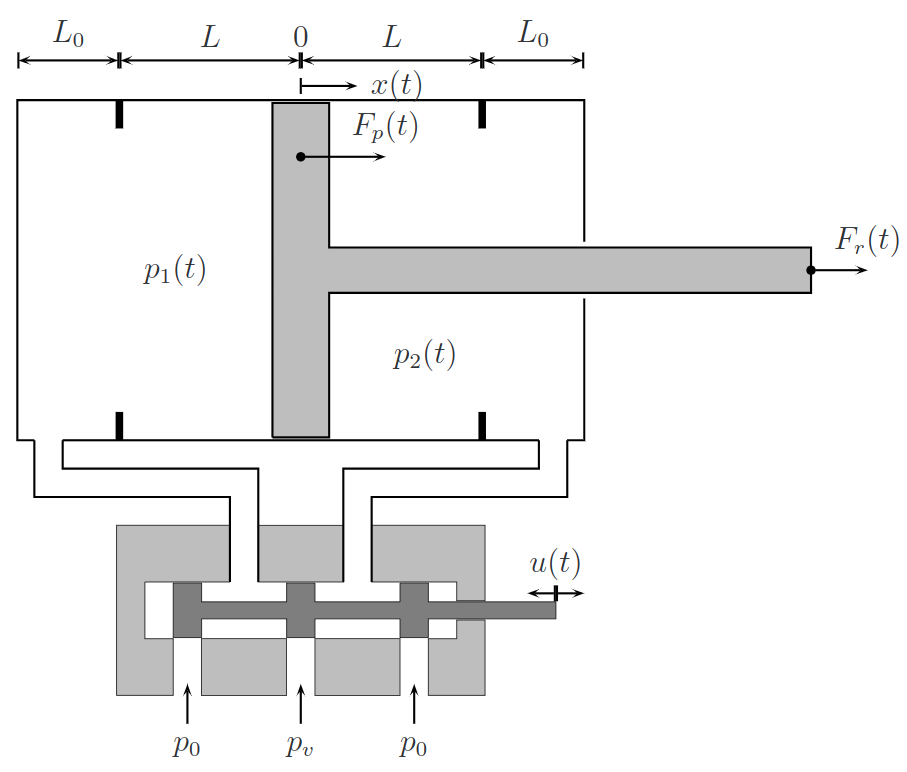
\includegraphics[width=0.6\linewidth]{../figures/pneumatic-cylinder.png}\\
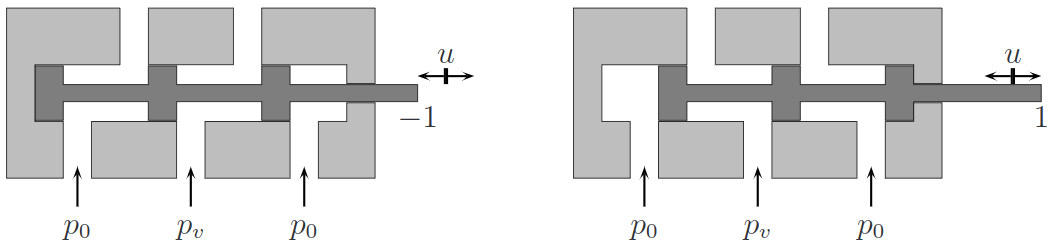
\includegraphics[width=0.7\linewidth]{../figures/pneumatic-valve.png}
\caption{A pneumatic cylinder. The input signal to the system $u(t)$ is the position of the valve. If $u$ is positive the valve core is displaced to the right (bottom right picture), then compressed air flows from the high-pressure inlet $p_v$ to the left chamber, while the air in the right chamber flows out. This causes an increase in the pressure difference $\Delta p(t) = p_1(t)-p_2(t)$. {\footnotesize From Ilchmann et al. ``Pneumatic cylinders: modelling and feedback force control'' Int Journal of Control, 2006}}
\label{fig:cylinder}
\end{center}
\end{figure}
We consider a linearized model about the operating point $\dot{x}_0=0$, $x_0=0$, $p_1=p_2=p$) and with  constant supply pressure $p_v$ and constant ambient pressure $p_0$. The flow through the valve is approximately proportional to the valve position $u$, which is the input signal to the system. The mass flows $\dot{m}_1$, $\dot{m}_2$ through the valve become
\[ \dot{m}_1 = \kappa u, \quad \dot{m}_2 = -\kappa u, \]
and the rate of change in pressures becomes
\begin{align}
  \dot{p}_1(t) &= \overbrace{k_uu}^{\text{flow in}} - \overbrace{k_{x}\dot{x}}^{\text{expansion}}\\
  \dot{p}_2(t) &= -k_{u}u + k_{x}\dot{x}.
\end{align}
The force $F(t)=F_r(t)$ of the cylinder equals the product of cross-sectional area $A$ of the piston and the difference in pressure between the two sides of the piston head.
\begin{equation}
  \frac{d}{dt} F(t) = \frac{d}{dt} A \Delta p(t) = -2Ak_{x}\dot{x}(t) + 2Ak_{u}u(t).
\end{equation}

The pneumatic cylinder is moving a mass $m$ subject to a disturbance force $v(t)$,  and we are neglecting any friction in the system. Let the velocity $y=\dot{x}$ be the output signal of the system. Newton's law \( m\ddot{x} = m\dot{y} = F+v\), differentiated once, gives 
\[ m\ddot{y} = \dot{F} + \dot{v} = -2Ak_{x}y + 2Ak_{u}u + \frac{d}{dt} v.\] The final model becomes
\begin{equation}
  \frac{d^2}{dt^2} y = -a y + bu + c\frac{d}{dt}v, 
  \label{eq:ode}
\end{equation}
where $a = \frac{2Ak_{x}}{m}$, $b=\frac{2Ak_{u}}{m}$ and $c = \frac{1}{m}$. 

\subsection*{Problems}

\begin{exercise}
 The model \eqref{eq:ode} can be written on transfer-function form as 
\begin{equation}
Y(s) = G(s)U(s) + G_d(s)V(s),
\label{eq:trf}
\end{equation}
where \( G(s) = \frac{b}{(s^2 + a)}. \)
Determine the transfer function $G_d(s)$.

\noindent
\fbox{
\bmpl
\textbf{ Calculations:}\\
\vspace*{50mm}
\emp}
\end{exercise}


\section*{Yaw control of a wind turbine}
Yaw is the angle between the direction the wind is blowing from and the direction the wind turbine is facing. Almost all wind turbines in commercial use have active control of the yaw angle in order to optimize energy production. \begin{center}
  \begin{tikzpicture}[node distance = 2cm]
    \node (image) {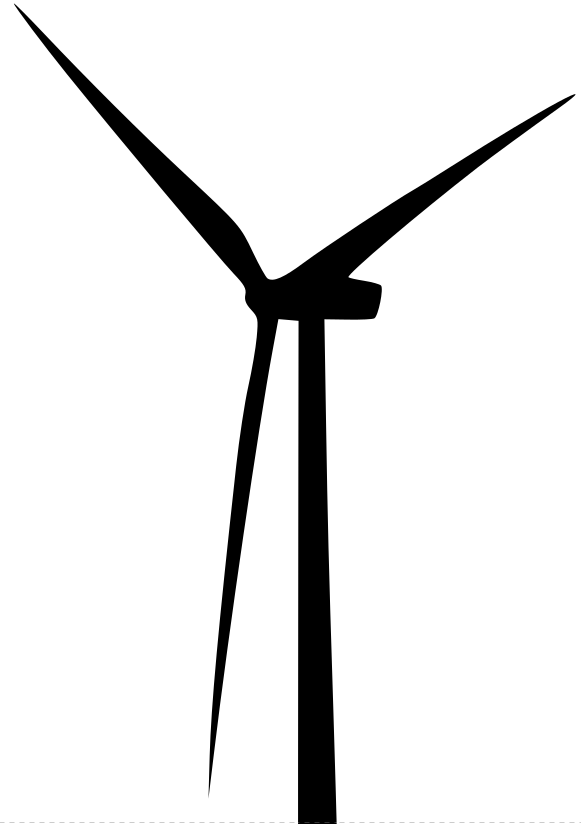
\includegraphics[width=0.2\linewidth]{../figures/wind-turbine-top.png}};
    \draw[->, thick, black!80!red!70] (1,0.65) -- node[coordinate, pos=0.8] (heading) {} (-3.4,0.65);
    \draw[->, thick, black!80!blue!70] (0.8,0.89) -- node[coordinate, pos=0.8] (winddir) {} (-2.7,-0.3);
    \draw[<-,] (heading) to[out=-135, in=150] node[left] {$y(t)$} (winddir);

    \node[coordinate, right of=image, node distance=5cm] (input) {};
    \node[circle, draw, inner sep=1pt, right of=input, ] (sum) {\small $\Sigma$};
    \node[draw, right of=sum, minimum height=12mm, minimum width=16mm] (block) {$G(s)$};
    \node[coordinate, right of=block] (output) {};
    \node[coordinate, above of=sum, node distance=14mm] (disturbance) {};
    
    \draw[->] (input) -- node[above, near start] {$u(t)$} (sum);
    \draw[->] (disturbance) -- node[left, near start] {$v(t)$} (sum);
    \draw[->] (sum) -- node[left, near start] {$$} (block);
    \draw[->] (block) -- node[above, near end] {$y(t)$} (output);
  \end{tikzpicture}
\end{center}
Assume that the friction force opposing the turning of the turbine is viscuous (proportional to the velocity), and that the wind force is causing a disturbance torque on the head. The dynamics of the system can then be described by the differential equation
\begin{equation}
 J\ddot{y}(t) + f\dot{y}(t) = u(t) + v(t),
\label{eq:odeyaw}
\end{equation}
where $y(t)$ is the yaw angle, $u(t)$ is the torque produced by the motor turning the head, $v(t)$ is the disturbance torque, $J$ is the moment of inertia and $f$ is the friction coefficient.

\subsection*{Problems}
\begin{exercise}

\abc
Show that the plant model \eqref{eq:odeyaw} can be expressed in the Laplace-domain as
\[ Y(s) = G(s)\big(U(s) + V(s)\big) = \frac{b}{s(s+a)} \big( U(s) + V(s)\big), \] 
with $b = \frac{1}{J}$ and $a = \frac{f}{J}$. 

\noindent
\fbox{
\bmpl
\textbf{Calculations:}\\
\vspace*{75mm}
\emp}

\abc
Choose a state vector $x$, and write the system \eqref{eq:odeyaw} on state-space form.
\begin{align*}
  \dot{x} &= Ax + B \bbm u\\v \ebm \\
  y &= Cx
\end{align*}

\noindent
\fbox{
\bmpl
\textbf{Calculations:}\\
\vspace*{75mm}
\emp}


\end{exercise}

\section*{A Coupled spring-mass system}
The figure below shows a system consisting of two masses connected together and to two rigid walls.
\begin{center}
  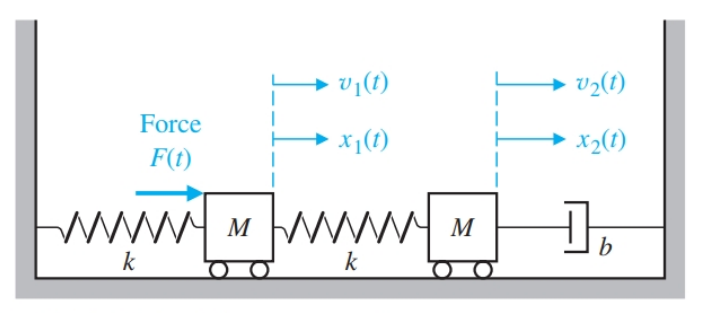
\includegraphics[width=0.55\linewidth]{../figures/DB-FigP2_3.png}
\end{center}
The displacements $x_1$ and $x_2$ are deviations from the equilibrium positions when the force acting on the left mass is zero. 

\subsection*{Problems}
\begin{exercise}
\abc
Determine the differential equations that describe the system.

\noindent
\fbox{
\bmpl
\textbf{ Calculations:}\\
\vspace*{50mm}
\emp}

\abc
Choose a suitable state vector $z$, and write the system on state-space form
\begin{align*}
  \dot{z}(t) &= Az(t) + B\,F(t)\\
  y(t) &= C z(t)
\end{align*}
where the interesting output is the position of the second mass, $y=x_2$.

\noindent
\fbox{
\bmpl
\textbf{ Calculations:}\\
\vspace*{80mm}
\emp}

\abc
The two springs are actually progressive, and the spring deflection (the relationship between spring force and length-change) can be described as
\begin{equation}
  F_s(x) = kx^3.
  \label{eq:deflection}
\end{equation}
Consider a situation in which the force acting on the left mass can be written as a deviation around a typical, positive value $F_0$
\[ F(t) = F_0 + u(t).\]
In equilibrium (steady-state) with constant $F(t) = F_0$, what is the position $x_1(t) = x_{0}$ in terms of the spring constant $k$ and the force $F_0$?

\noindent
\fbox{
\bmpl
\textbf{ Calculations:}\\
\vspace*{50mm}
\emp}


\abc
Determine the constant $a$ in the linearized model
\begin{equation}
v = aw, \quad \text{where} \; F_s = F_0 + v,\; x_1 = x_{0} + w 
\end{equation}
for the left-most spring with operating point $(F_0, x_{0})$

\noindent
\fbox{
\bmpl
\textbf{ Calculations:}\\
\vspace*{50mm}
\emp}
\end{exercise}



\cleardoublepage
%\end{document}
\section*{Solutions}
\setcounter{exerctr}{0} 

\subsection*{Pneumatic cylinder}
\begin{exercise}
 Taking the Laplace transform of each term in the model \eqref{eq:ode}, and setting all initial values to zero (we are interested in the transfer function, not the transient response to the initial value) gives
\[ s^2 Y(s) = -aY(s) + bU(s) + csV(s),\]
which solved for $Y(s)$ is
\[ Y(s) = \frac{b}{s^2 + a} U(s) + \frac{cs}{s^2 + a} V(s).\]
Hence \[G_d(s) = \frac{cs}{s^2 + a}.\]
\end{exercise}

\subsection*{Wind turbine}

\begin{exercise}
  \abc
  Since we are interested in the transfer function only, not the response to initial values, we set all initial values to zero when applying the Laplace transform to \eqref{eq:odeyaw}. This gives
  \[Js^2Y(s) + fsY(s) = U(s) + V(s)\]
  solving for Y(s) gives
  \[ Y(s) = \frac{\frac{1}{J}}{s(s+\frac{f}{J})} U(s) + \frac{\frac{1}{J}}{s(s+\frac{f}{J})}V(s) = \frac{\frac{1}{J}}{s(s+\frac{f}{J})}(U(s) + V(s)) \]

  \abc
  One suitable choice of state vector is
  \[ x = \bbm y\\\dot{y} \ebm, \]
  which gives the model
  \begin{align*}
    \dot{x}_1 &= \dot{y} = x_2\\
    \dot{x}_2 &= -\frac{f}{J}\dot{y} + \frac{1}{J} u + \frac{1}{J} v = -\frac{f}{J}x_2 + \frac{1}{J}u + \frac{1}{J} v
  \end{align*}
  which can be written
  \begin{align*}
    \dot{x} &= \bbm 0 & 1\\0 & -\frac{f}{J} \ebm x + \bbm 0 & 0 \\\frac{1}{J} & \frac{1}{J}  \ebm \bbm u\\v\ebm.\\
    y &= \bbm 1 & 0 \ebm x.
  \end{align*}

\end{exercise}

\subsection*{Spring-mass system}

\begin{exercise}
  \abc
  Free-body-diagrams of the two bodies gives
  \begin{center}
    \begin{tikzpicture}
      \node[draw, minimum height=14mm, minimum width=14mm] (m1) {M};
      \draw[->] (m1.west) -- ++(-14mm, 0) node[below] {$F_{s_1}$};
      \draw[<-] (m1.north west) -- ++(-14mm, 0) node[above] {$F$};
      \draw[<-] (m1.east) -- ++(14mm, 0) node[above] {$F_{s_2}$};

      \begin{scope}[xshift = 6cm]
      \node[draw, minimum height=14mm, minimum width=14mm] (m2) {M};
      \draw[<-] (m2.west) -- ++(-14mm, 0) node[above] {$F_{s_2}$};
      \draw[<-] (m2.east) -- ++(14mm, 0) node[above] {$F_{d}$};
      \end{scope}
    \end{tikzpicture}
  \end{center}
  where the spring forces are given by
  \[ F_{s_1} = kx_1, \qquad F_{s_2} = k(x_1-x_2), \]
  and the damper force
  \[ F_d = b \dot{x}_2\]
  Newton's second law for each body gives
  \begin{align*}
    M\ddot{x}_1 &= F - F_{s_1} - F_{s_2} = F - kx_1 - k(x_1-x_2)\\
    M\ddot{x}_2 &=   F_{s_2} -F_d = k(x_1-x_2) - b\dot{x}_2.
  \end{align*}

  \abc
  One choice of state vector is
  \[ z = \bbm x_1\\ \dot{x}_1 \\x_1-x_2 \\dot{x}_2 \ebm, \]
  with which the differential equations can be written
  \begin{align*}
    \dot{z}_1 &= \dot{x}_1 = z_2\\
    \dot{z}_2 &= \ddot{x}_1 = -\frac{k}{M} x_1 - \frac{k}{M}(x_1-x_2) + \frac{1}{M} F = -\frac{k}{M}z_1  -\frac{k}{M}z_3  + \frac{1}{M} F\\
    \dot{z}_3 &= \dot{x}_1 - \dot{x}_2 = z_2 - z_ 4\\
    \dot{z}_4 &= \ddot{x}_2 = \frac{k}{M}(x_1 - x_2) - \frac{b}{M}\dot{x}_2 = \frac{k}{M}z_3 - \frac{b}{M}z_4. 
  \end{align*}
  The state-space model becomes
  \begin{align*}
    \dot{z} &= \bbm 0 & 1 & 0 & 0\\ -\frac{k}{M} & 0 & -\frac{k}{M} & 0 \\ 0 & 1 & 0 & -1\\ 0 & 0 & \frac{k}{M} & -\frac{b}{M} \ebm z + \bbm 0\\\frac{1}{M}\\0\\0\ebm\\
    y &= x_2 = \bbm 1 & 0 & -1 & 0\ebm z.
  \end{align*}

  \abc
  In equilibrium with a constant force $F(t)=F_0$, the masses will be shifted to the right a distance $x_1=x_2=x_0$. For the left-most mass, we get that, since $\ddot{x}_1 = 0$ and the forces are in balance,
  \[ 0 = F_0 -F_s = F_0 - kx_0^3.\]
  Solving for $x_0$ gives
  \[ x_0 = \left(\frac{F_0}{k}\right)^\frac{1}{3}. \]

  \abc
  The Taylor-expansion of $F_s(x_1) = kx_1^3$ about the point $x_0$ is given by
  \[ F_s(x_1) = F_s(x_0) + 3kx_0^2 (x_1-x_0) + \frac{6kx_0}{2!}(x_1-x_0)^2 + \frac{6k}{3!}(x_1-x_0)^3,\]
  so the linear model becomes
  \[ F_s(x_1) \approx F_s(x_0) + 3kx_0^2(x_1-x_0) = F_0 + 3kx_0^2 w\]
  \[ F_s - F_0 = 3kx_0^2 w\]
  \[ v = 3kx_0^2 w.\]
  The parameter we are looking for is
  \[ a = 3kx_0^2 = 3k\left(\big(\frac{F_0}{k}\big)^\frac{1}{3}\right)^2 = 3k\big(\frac{F_0}{k}\big)^\frac{2}{3} =  3k^\frac{1}{3}F_0^\frac{2}{3}. \]
  
\end{exercise}
\end{document}
